


%	PACKAGES AND OTHER DOCUMENT CONFIGURATIONS

\documentclass[
	12pt, % Default font size, values between 10pt-12pt are allowed
	%letterpaper, % Uncomment for US letter paper size
	%spanish, % Uncomment for Spanish
]{style/fphw}

% Template-specific packages

\usepackage[utf8]{inputenc} % Required for inputting international characters
\usepackage[T1]{fontenc} % Output font encoding for international characters
\usepackage{mathpazo} % Use the Palatino font
\usepackage{amssymb}
\usepackage{graphicx} % Required for including images
\usepackage{booktabs} % Required for better horizontal rules in tables
\usepackage{listings} % Required for insertion of code
\usepackage{enumerate} % To modify the enumerate environment
\usepackage{epstopdf}
% \epstopdfDeclareGraphicsRule{.tif}{png}{.png}{convert #1 \OutputFile}
\AppendGraphicsExtensions{.tif}
\usepackage[ruled,vlined]{algorithm2e}
\usepackage{minted}
\usepackage[nottoc]{tocbibind}
\usepackage{caption}
\usepackage{subcaption}
\usepackage{mathtools}
\DeclarePairedDelimiter\abs{\lvert}{\rvert}%
\DeclarePairedDelimiter\norm{\lVert}{\rVert}%

% Swap the definition of \abs* and \norm*, so that \abs
% and \norm resizes the size of the brackets, and the 
% starred version does not.
\makeatletter
\let\oldabs\abs
\def\abs{\@ifstar{\oldabs}{\oldabs*}}
%
\let\oldnorm\norm
\def\norm{\@ifstar{\oldnorm}{\oldnorm*}}
\makeatother





%----------------------------------------------------------------------------------------
%	ASSIGNMENT INFORMATION
%----------------------------------------------------------------------------------------

\title{Lab 4 Frquency Domain Filtering} % Assignment title

\author{YUAN Tong 11810818} % Student name

%\date{March 28th, 2025} % Due date

\institute{Southern University of Science and Technology \\ School of Microelectronic} % Institute or school name

\class{LAB Session I} % Course or class name

\professor{YU Yajun} % Professor or teacher in charge of the assignment

%----------------------------------------------------------------------------------------

\begin{document}
\definecolor{bg}{rgb}{0.95,0.95,0.95}
\maketitle % Output the assignment title, created automatically using the information in the custom commands above

%----------------------------------------------------------------------------------------
%	ASSIGNMENT CONTENT
%----------------------------------------------------------------------------------------

\section*{Introduction}

A thorough understanding of image filtering is impossible without having at least a working knowledge of how the Fourier transform and the frequency domain can be used for image filtering. Briefly, the frequency domain is a space which is defined by \textbf{Fourier Transform} -- a very wide application in image processing, \textbf{frequency domain analysis} is used to indicate how signal energy can be distributed in a range of frequency. By filtering in frquency domain, we can manipulate signal with specific frquency contianed in the image.

In this LAB, we will first introduce the procedure by which we used to apply Discrete Fourier Transform to image and different kinds of operator, then we will apply \textbf{soble}, \textbf{Gaussian} and \textbf{Butterworth} notch filters to differnt image and analysis their performance.

Gengrally, this serises of methods can be used to extract specific imformation contained in the image, can sharp or unshape the image, pre-process the image for neural network training, and also can add special effect to the iamge. As the most widely used technic for image processing, Fourier Transform still benifits many areas.

\newpage

\section*{Fourier Transform and Filtering in Frquency Domain}

\subsection*{Fourier Transform Basic} \

In 1D case, we demostrate that all converage continous signal can be writen in the form of $$f(t)=\sum_{n=-\infty}^{+\infty}$$ with $$c_n=\frac{1}{T} \int_{-T/2}^{T/2}f(t)e^{j\frac{2\pi n}{T}t}$$ and we define fourier transform as $$F(\mu) = \Im\{f(t)\} = \int_{-\infty}^{\infty}f(t)e^{j2\pi \mu t} $$

One important property of fourier transform is that the Fourier transform of the convolution of two functions in the spatial domain is equal to the product in the frequency domain of the Fourier transforms of the two functions, and can be expressed as $$f(t)\bigstar h(t)=H(\mu)F(\mu)$$ or $$f(t) h(t)=H(\mu) \bigstar F(\mu)$$ which will be the basic idea in Frquency domain filtering.

For arbitery discrete signal, we have $$F(u) = \sum_{n=0}^{M-1}f_n e^{-j2\pi un/M}$$ and $$f(x)=\frac{1}{M} \sum_{u=0}^{M-1} F(u)e^{j2\pi ux/M}$$ with property $$F(u)=F(u+kM)$$

\subsection*{Fourier Transform For Image} \

To apply Fourier tranform to image, firstly we need to expand the Fourier Transform to 2D form. The 2D fourier transform can be expressed as $$F(\mu,\nu)=\int_{-\infty}^{+\infty}\int_{-\infty}^{+\infty}f(t,z)e^{-j2\pi (\mu t + \nu z)}dtdz$$ and $$f(u,v)=\int_{-\infty}^{+\infty}\int_{-\infty}^{+\infty}F(\mu,\nu)e^{j2\pi (\mu t + \nu z)}d\mu d\nu$$ 

And in decrete form we have $$F(u,v)= \sum_{x=0}^{M-1}\sum_{y=0}^{N-1}f(x,y)e^{-j2\pi (ux/M + vy/N)}$$ and $$f(x,y)=\frac{1}{MN}\sum_{x=0}^{M-1}\sum_{y=0}^{N-1}F(u,v)e^{-j2\pi (ux/M + vy/N)}$$

\subsection*{Image Filtering in Frquency domain} \

\subsubsection*{Property}

Several important properties of Fourier Transform will be introduced here so we can design the procedure of the image processing steps.

\textbf{Firstly}, is the relationship that $$f(t)\bigstar h(t)=H(\mu)F(\mu)$$ or $$f(t) h(t)=H(\mu) \bigstar F(\mu)$$ which we have introduced before, according to this property we can first do the Fourier Transform to both image and the operator, multiple them together, and than do the reverse Fourier Transform to the product, the result is the image filtered in frquency domain. 

\textbf{Secondly} is about the periodicity, we have $$f(x)e^{j2\pi (u_0x/M)} \Leftrightarrow F(u-u_0)$$ we assign $u_0 = \frac{M}{2}$ to the fomular and we obtain $$f(x)(-1)^{x} \Leftrightarrow F(u-M/2)$$ and for 2D we have $$f(x,y)(-1)^{x+y} \Leftrightarrow F(u-M/2, v-N/2)$$ the result of such transform are shown in Figure \ref{shift.png} The periodicities of the transform and its inverse are important issues in the implementation of DFT-based algorithms. the transform data in the interval from 0 to M - 1 consists of two back-to-back half periods meeting at point M/2. Shift the zero-frequency component to the center of the spectrum \textbf{For display and filtering purposes}, it is more convenient to \textbf{have in this interval a complete period of the transform} in which the data are contiguous. If we do not perform the shift operation, we will get the result shown in Figure \ref{Q5_2_lowpass_30_error.tif}

\begin{figure}[H]
    \centering
    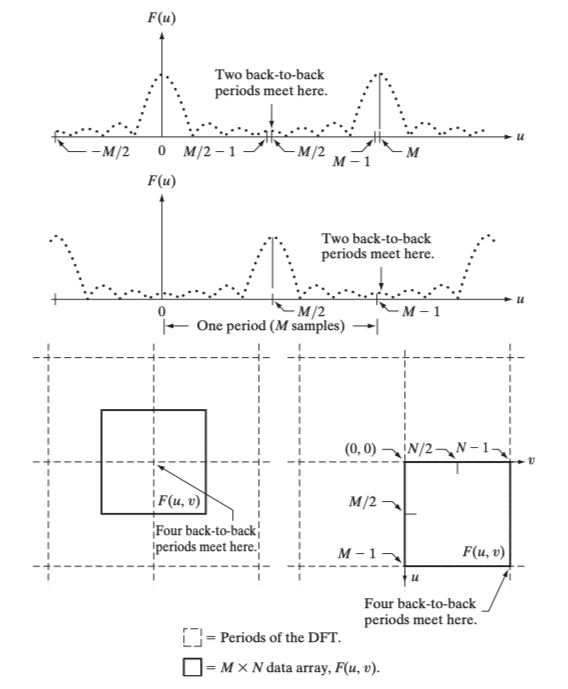
\includegraphics[width=0.6\linewidth]{chart/shift.png}
    \caption{Shifting of the signal}
    \label{shift.png}
\end{figure}

\textbf{Thirdly}, and most importantly, is about the Symmetry Properties, we define decrete function that satisfy $f(x)=f(N - x)$ even function and those satisfy $f(x)= -f(N - x)$ odd function.

\subsubsection*{Zero padding}

Before we apply the Fourier Transform to the iamge, we will first pad the image as shown in Figure \ref{padding.png}. Because we are dealing here with discrete quantities, computation of the Fourier transforms is carried out with a DFT algorithm. If we elect to compute the spatial convolution using the IDFT of the product of the two transforms, then the periodicity issues must be taken into account. when convolving two periodic functions, the convolution itself is periodic, so we may meet wraparound error as shown in Figure \ref{wraparound error}, so to avoid this we must pad the image with the $$P > A + C - 1$$ and $$Q > B + D - 1$$ with $$P > 2M - 1$$ and $$Q > 2N - 1$$

\begin{figure}[H]
     \centering
     \begin{subfigure}[b]{0.2\textwidth}
         \centering
         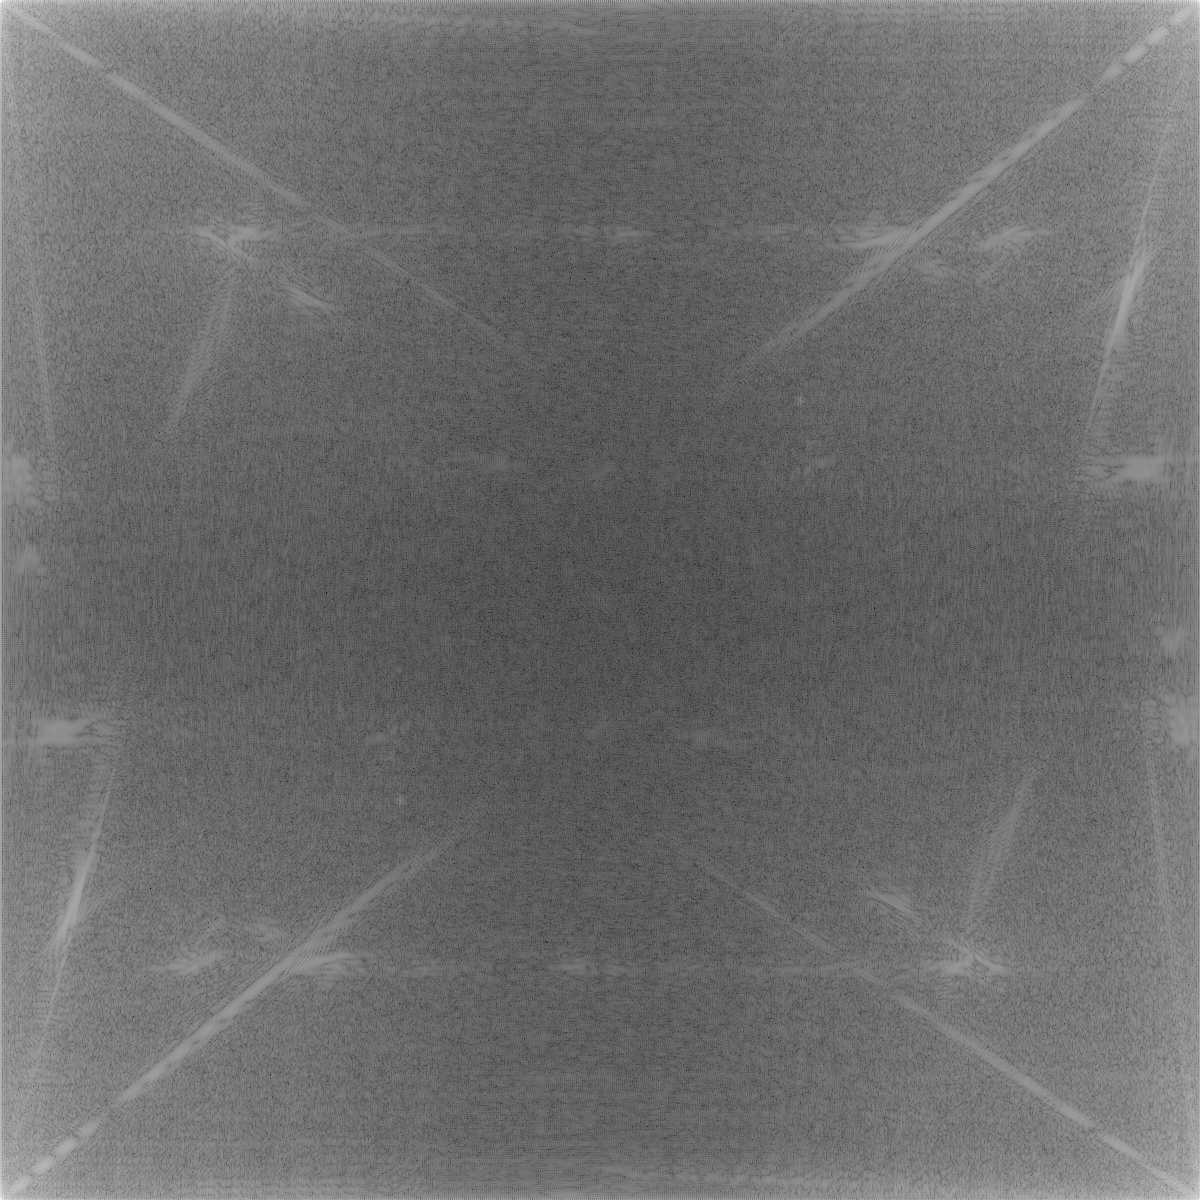
\includegraphics[width=\textwidth]{plots2/Q5_1_spectrum_noshift.png}
         \caption{without shift}
         \label{Q5_2_lowpass_30_error.tif}
     \end{subfigure}
     \hfill
     \begin{subfigure}[b]{0.2\textwidth}
         \centering
         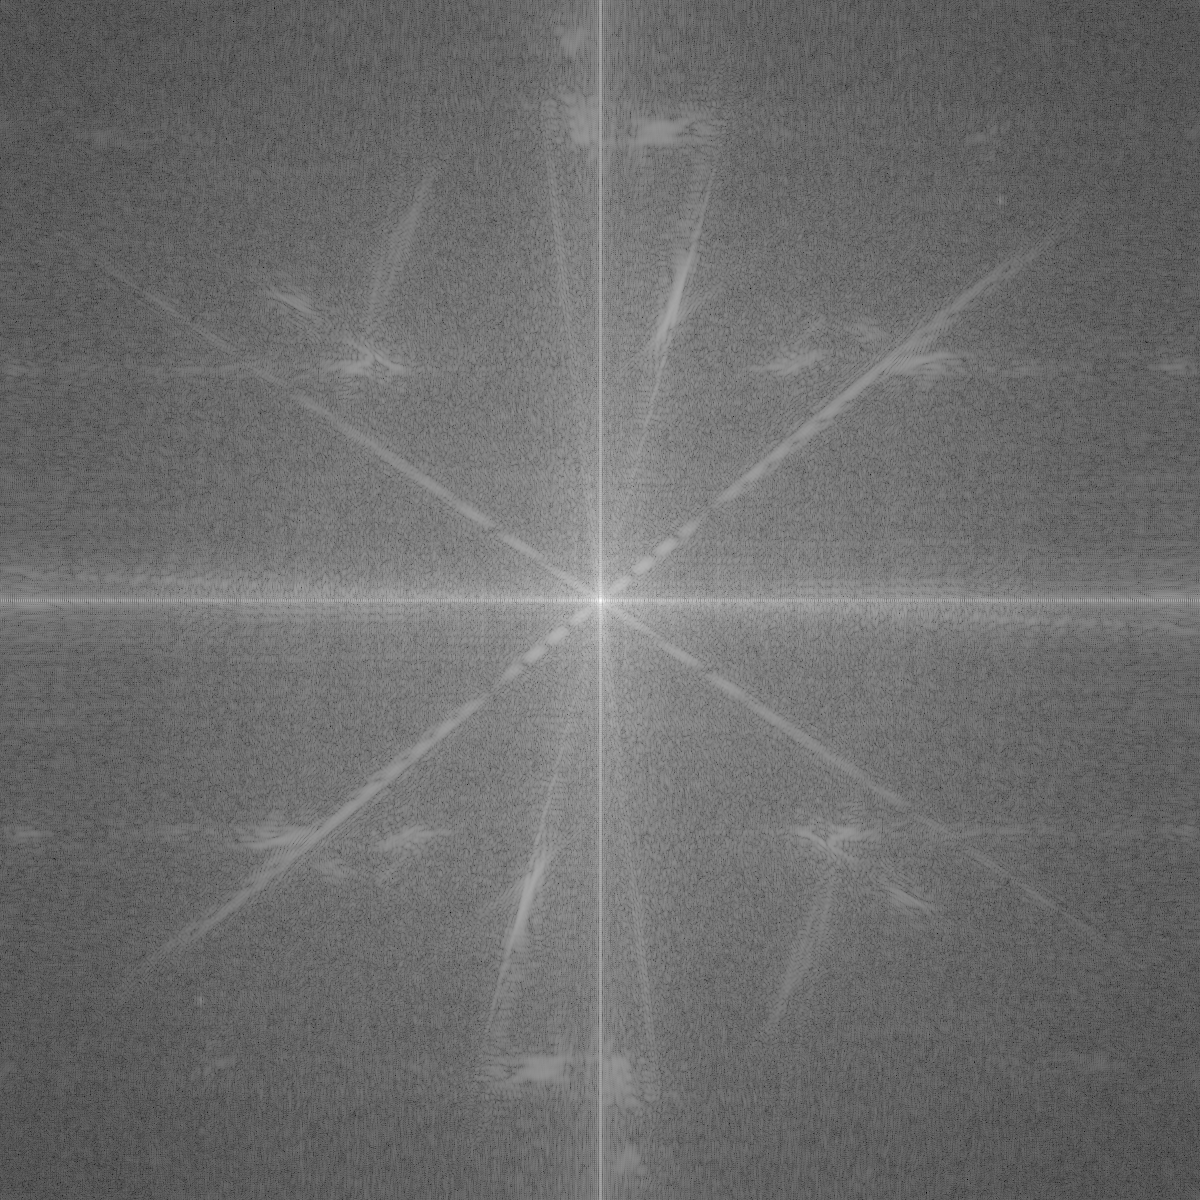
\includegraphics[width=\textwidth]{plots2/Q5_1_spectrum.png}
         \caption{with shift}
         \label{Q5_2_lowpass_30_error.tif}
     \end{subfigure}
     \hfill
     \begin{subfigure}[b]{0.2\textwidth}
         \centering
         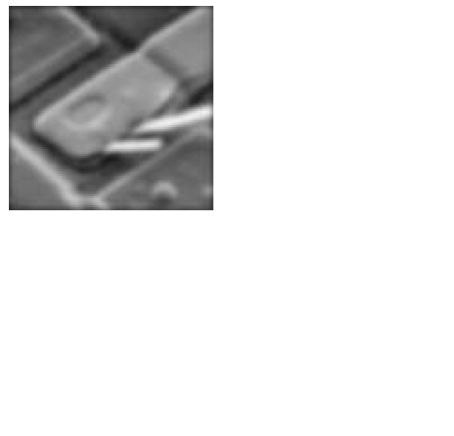
\includegraphics[width=\textwidth]{chart/padding.png}
         \caption{Padding}
         \label{padding.png}
     \end{subfigure}
     \hfill
     \begin{subfigure}[b]{0.2\textwidth}
         \centering
         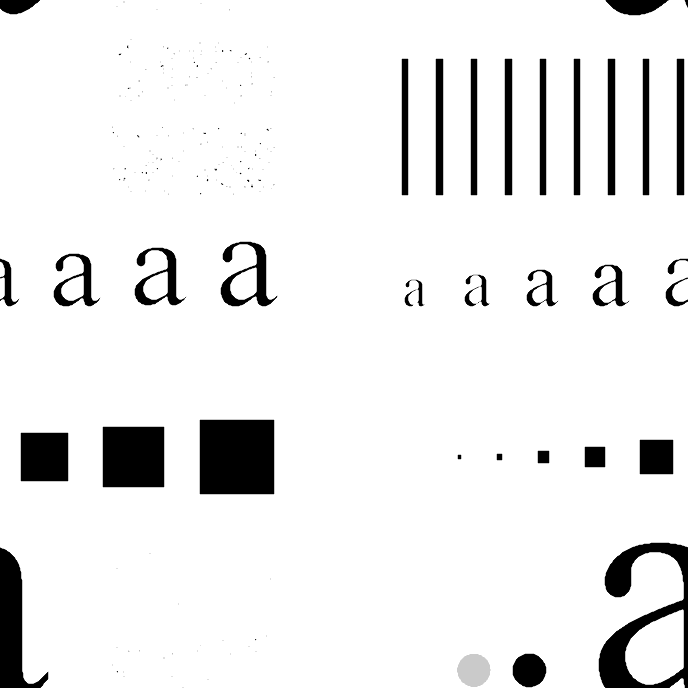
\includegraphics[width=\textwidth]{plots/warpped.png}
         \caption{error}
         \label{wraparound error}
     \end{subfigure}
        \caption{Why we need padding and shift}
        \label{padding}
\end{figure}

\subsubsection*{Procedure}
Here we summrize the steps to filtering in frquency domain

\begin{enumerate}
    \item Given an input image $f(x,y)$ of size $M \times N$, obtain the padding parameters P and Q. Typically, P = 2M and Q = 2N.
    \item Form a padded image, $f_p(x,y)$ of size $P \times Q$ by appending the necessary number of zeros to $f(x,y)$
    \item Multiply $f_p(x,y)$ by $(-1)^{x+y}$ to center its transform
    note: as mentioned in property 2, centering helps in visualizing the filtering process and in generating the filter functions themselves, but centering is not a fundamental requirement.
    \item Compute the DFT, F(u,v) of the image from step 3 
    \item Generate a real, symmetric filter function, $H(u,v)$, of size $P \times Q$ with center at coordinates $(P/2, Q/2)$
    \item Form the product $G(u,v) = H(u,v)F(u,v)$ using array multiplication
    \item Obtain the processed image $$g_p(x, y)=\{real[\Im^-1 [G(u, v)]] \}(-1)^{x+y}$$ 
    \item Obtain the final processed result, $g(x,y)$, by extracting the $M \times N$ region from the top, left quadrant of $g_p(x,y)$
\end{enumerate}


\newpage
\section*{Task 1: Sobel filter}

\begin{problem}
	Implement the Sobel filter to the input images Q5\_1.tif in both spatial domain and frequency domain. Compare the results. Refer to slides 78 to 81 of Lecture 4.
	\begin{figure}[H]
	    \centering
	    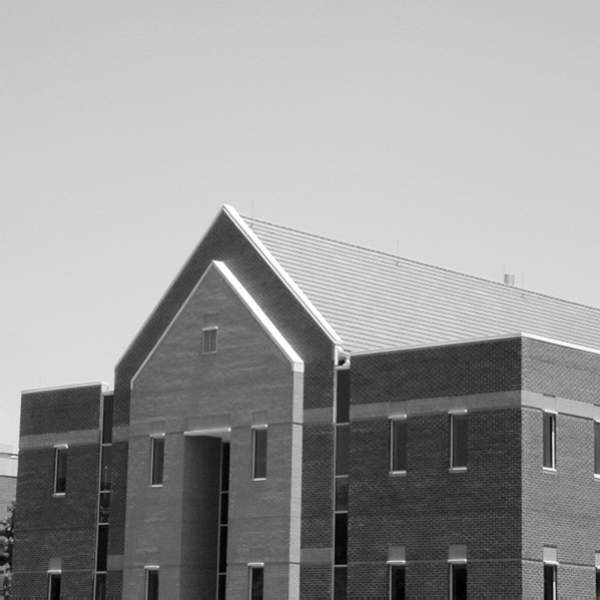
\includegraphics[width=0.3\linewidth]{plots/Q5_1.png}
	    \caption{Q5\_1.tif}
	    \label{Q5_1.tif}
	\end{figure}
\end{problem}

\subsection*{Analysis}

The Sobel operator is used in image processing and computer vision, particularly within \textbf{edge detection} algorithms where it creates an image emphasising edges. The application of Sobel opeartor can be write as $$ \textbf{G}_x = \left[\begin{array}{ccc}
    +1 & 0 & -1 \\
    +2 & 0 & -2 \\
    +1 & 0 & -1 
\end{array}\right] \ast A $$ and $$ \textbf{G}_y = \left[\begin{array}{ccc}
    +1 & +2 & +1 \\
    0 & 0 & 0 \\
    -1 & -2 & -1 
\end{array}\right] \ast A $$

In this task we will apply both vertal and horizontal filter to the given image to detect the eage contained in the image on both spatal domain and frquency domain.

And to apply a spatal filter to frquency domain, we need to do the step 2 to 4 in the basic steps of image processing in frquency domain, then multiply them together, finally we do IDFT to the product and we can get the result.

\subsection*{Result} \

In this task we first apply the sobel filter to the image in spatal domain, and we get the result shown in Figure \ref{Q5_1_spatial.png}.

Then we apply the sobel operator on frquency domain, first convert the image by shift and DFT to frquency domain as shown in Figure \ref{Q5_1_spectrum.png}, second, we apply same procedure to the sobel filter after padding it and we obtain Figure \ref{Q5_1_filter.png}, finally we multiply then together and get Figure \ref{Q5_1_frequency.png}, compare Figure \ref{Q5_1_spatial.png} and Figure \ref{Q5_1_frequency.png}, we found that they are almost the same, which means here filter in spatal domain and filter in frequence domain are equal.
 
\begin{figure}[H]
     \centering
     \begin{subfigure}[b]{0.45\textwidth}
         \centering
         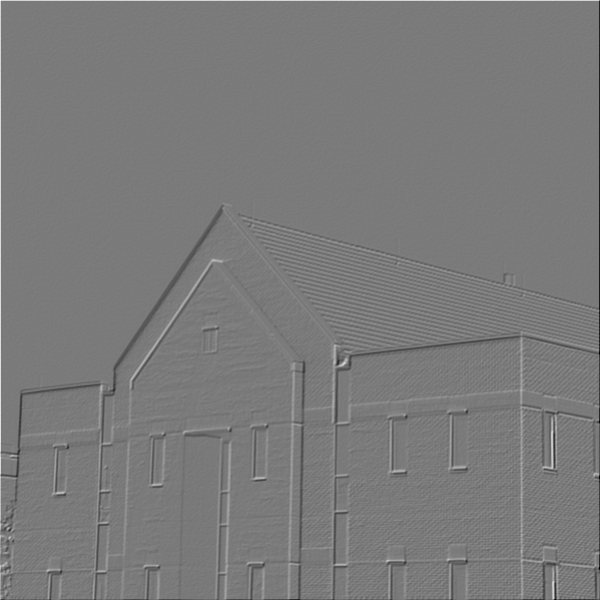
\includegraphics[width=\textwidth]{plots2/Q5_1_spatial.png}
         \caption{spatal}
         \label{Q5_1_spatial.png}
     \end{subfigure}
     \hfill
         \begin{subfigure}[b]{0.45\textwidth}
         \centering
         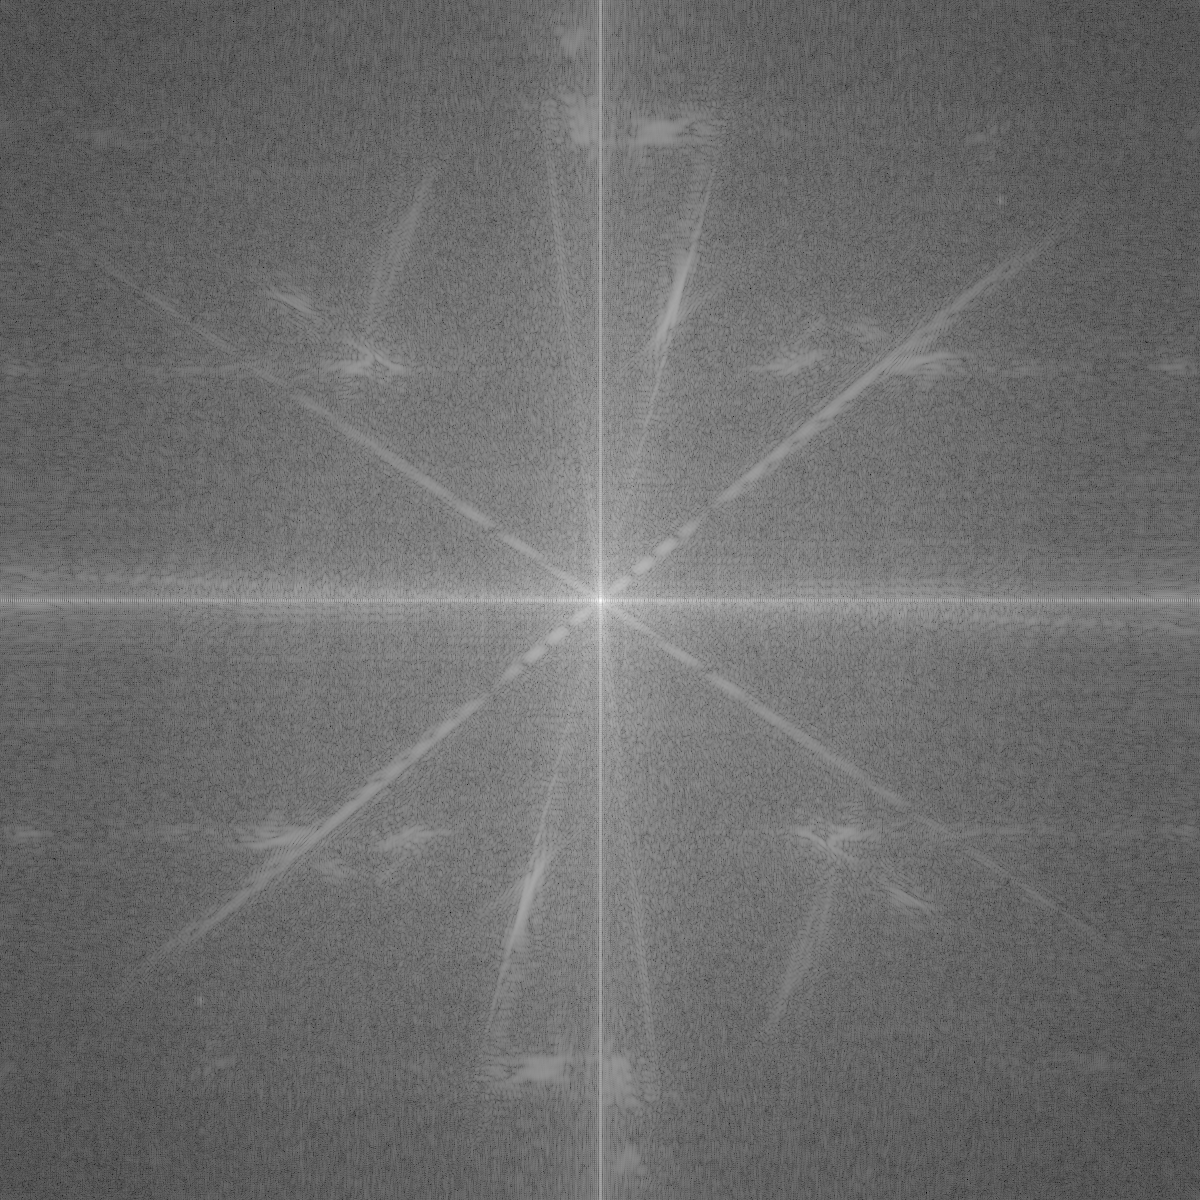
\includegraphics[width=\textwidth]{plots2/Q5_1_spectrum.png}
         \caption{spectrum}
         \label{Q5_1_spectrum.png}
     \end{subfigure}
     \vfill
     \begin{subfigure}[b]{0.45\textwidth}
         \centering
         
\includegraphics[width=\textwidth]{plots2/Q5_1_filter.png}
         \caption{Filter}
         \label{Q5_1_filter.png}
     \end{subfigure}
     \hfill
     \begin{subfigure}[b]{0.45\textwidth}
         \centering
         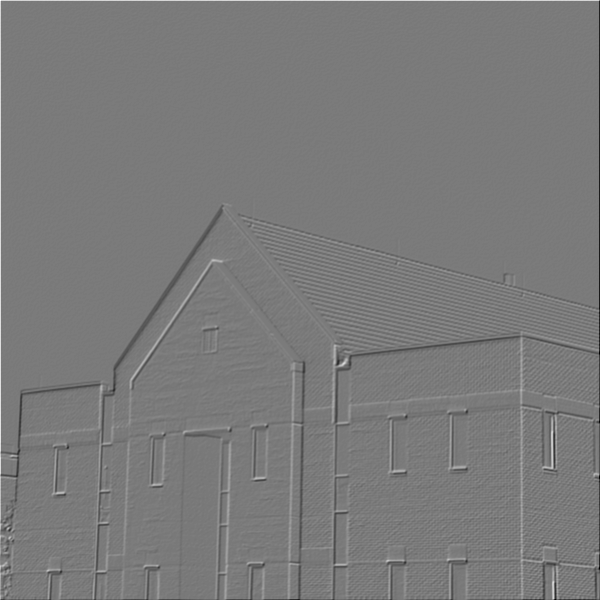
\includegraphics[width=\textwidth]{plots2/Q5_1_frequency.png}
         \caption{frquency}
         \label{Q5_1_frequency.png}
     \end{subfigure}
        \caption{Image filtered by sobel filter in spatal domain}
        \label{sobel filter spatal}
\end{figure}

\subsection*{Discussion}

In this task we apply a shift at the step 4, and the reason has been discussed at last session.

And there is another rules that in both procedure, if you filp the sobel operator we can found the output image also "flipped", the "direction" of the gridant in both image will change.

\newpage
\section*{Task 2: Gaussian low pass and high pass}

\begin{problem}
Implement the Gaussian low pass and high pass to the input image Q5\_2.tif. results for $D_0$ 0 = 30 , 60 , and 160, respectively.

\begin{figure}[H]
    \centering
    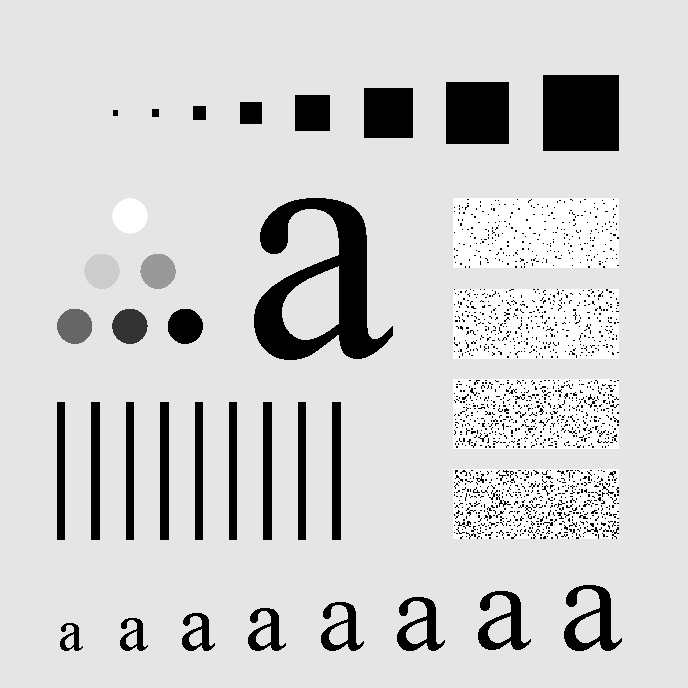
\includegraphics[width=0.3\linewidth]{plots/Q5_2.png}
    \caption{Q5\_2.tif}
    \label{Q5_2.tif}
\end{figure}
\end{problem}

\subsection*{Analysis} \

In this task, our goal is to reduce the signal intensity contianed in high or low frquency domain by Gaussian filter. The Gaussian filter can be described as $$H(u,v)=e^{-D^2(u,v)/2\sigma^2}$$ as shown in Figure \ref{Gaussian.png}, bigger n is, less signal in high frquency will be filtered.

\begin{figure}[H]
    \centering
    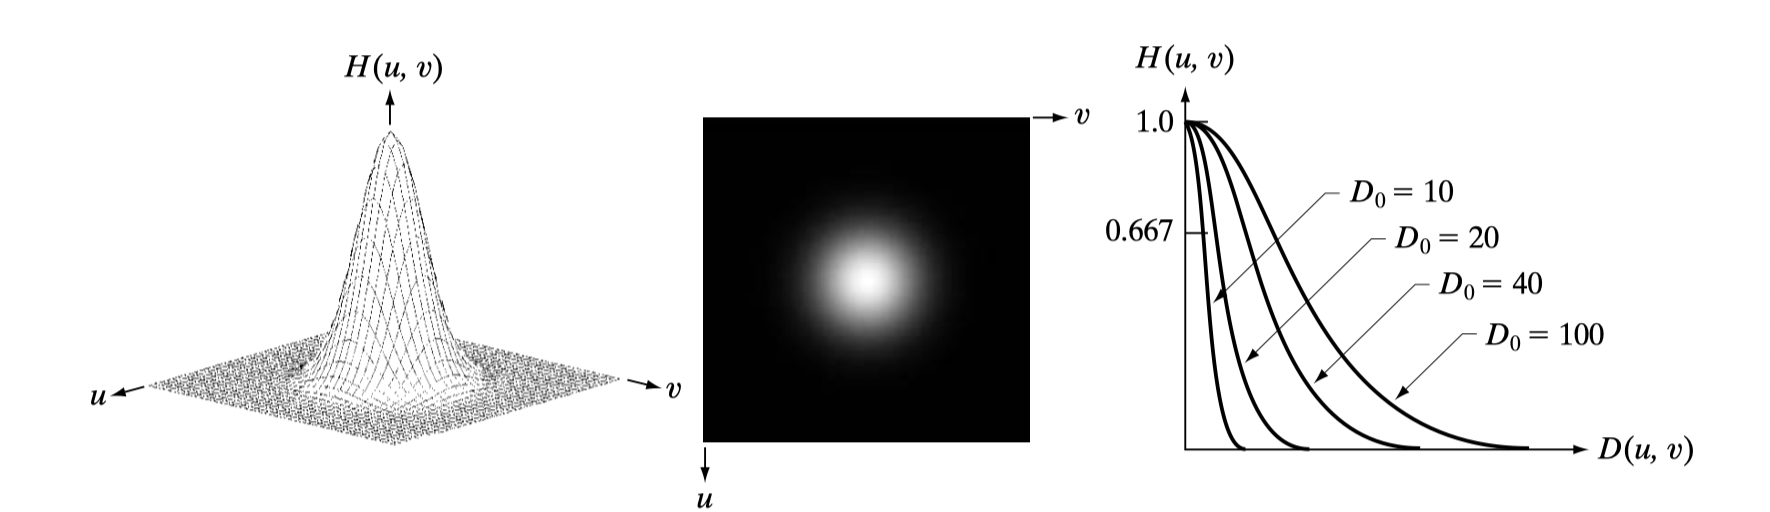
\includegraphics[width=0.8\linewidth]{chart/Gaussian.png}
    \caption{Gaussian lowpass filter}
    \label{Gaussian.png}
\end{figure}

\subsection*{Result} \

In this task, we apply Gaussian highpass and lowpass filter with $\sigma$ equal to 30, 60, 160, the Gaussian lowpass filters and the filtered images are shown in Figure \ref{Gaussian low filter}

\begin{figure}[H]
    \centering
     \begin{subfigure}[b]{.3\textwidth}
         \centering
         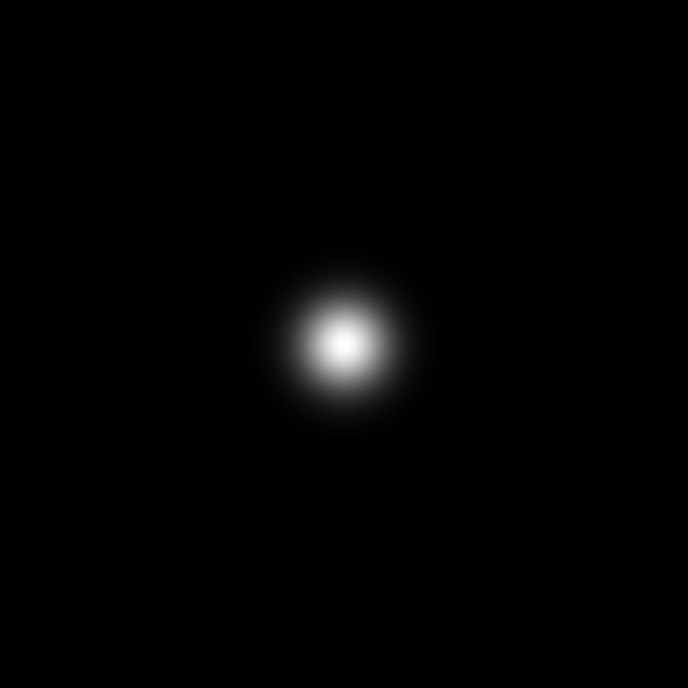
\includegraphics[width=\textwidth]{plots2/Q5_2_lowpass_filter_30.png}
         \caption{$\sigma=30$}
         \label{Q5_2_lowpass_filter_30}
     \end{subfigure}
     \hfill
     \begin{subfigure}[b]{.3\textwidth}
         \centering
         
\includegraphics[width=\textwidth]{plots2/Q5_2_lowpass_filter_60.png}
         \caption{$\sigma=60$}
         \label{Q5_2_lowpass_filter_60}
     \end{subfigure}
     \hfill
     \begin{subfigure}[b]{.3\textwidth}
         \centering
         
\includegraphics[width=\textwidth]{plots2/Q5_2_lowpass_filter_160.png}
         \caption{$\sigma=160$}
         \label{Q5_2_lowpass_filter_160}
     \end{subfigure}
     \vfill
     \begin{subfigure}[b]{.3\textwidth}
         \centering
         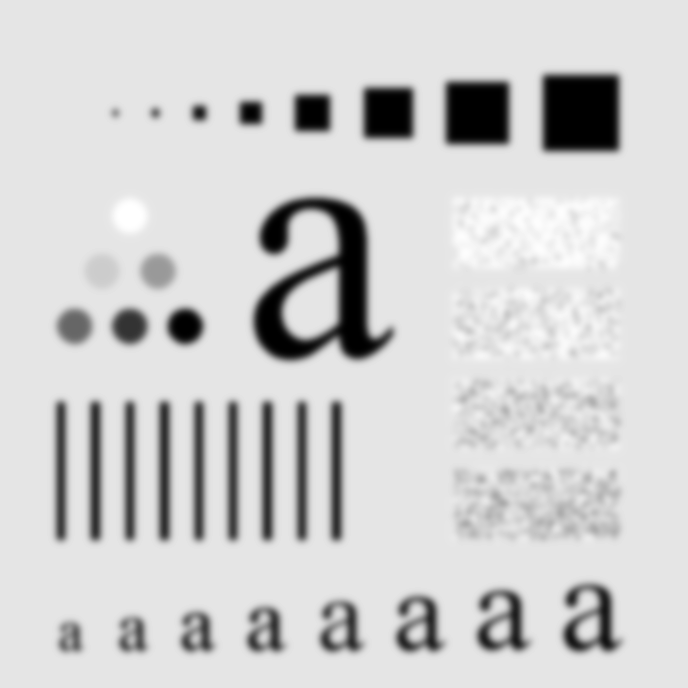
\includegraphics[width=\textwidth]{plots2/Q5_2_lowpass_30.png}
         \caption{$\sigma=30$}
         \label{Q5_2_lowpass_30}
     \end{subfigure}
     \hfill
     \begin{subfigure}[b]{.3\textwidth}
         \centering
         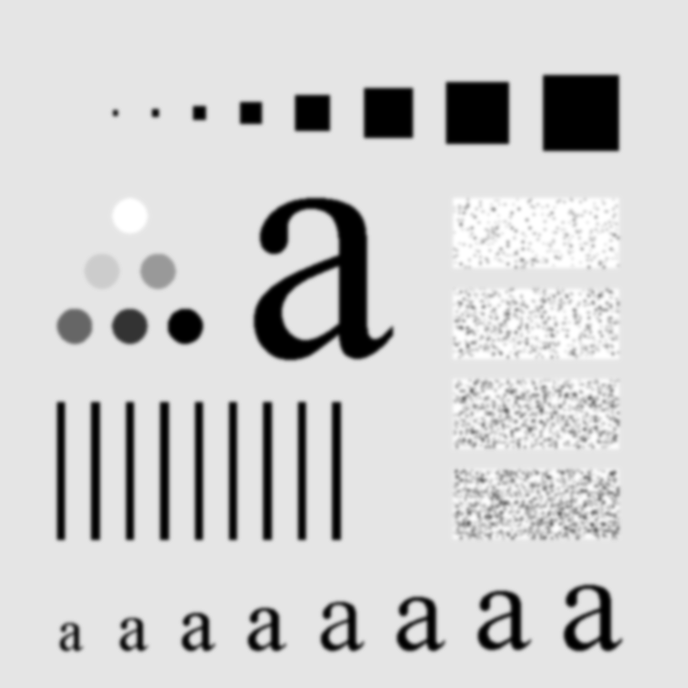
\includegraphics[width=\textwidth]{plots2/Q5_2_lowpass_60.png}
         \caption{$\sigma=60$}
         \label{Q5_2_lowpass_60}
     \end{subfigure}
     \hfill
     \begin{subfigure}[b]{.3\textwidth}
         \centering
         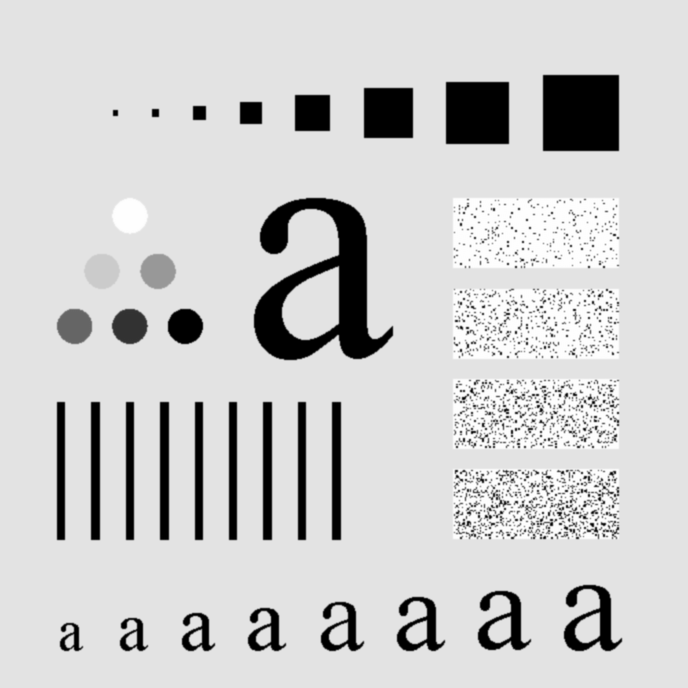
\includegraphics[width=\textwidth]{plots2/Q5_2_lowpass_160.png}
         \caption{$\sigma=160$}
         \label{Q5_2_lowpass_160}
     \end{subfigure}
     
    \caption{The Gaussian low filter and output images}
    \label{Gaussian low filter}
\end{figure}

Here we can found that, as $\sigma$ increase, the image become clearer, which means that more infromation in high frequency domain is reserved, and the image is sharper.

Then we convert Gaussian lowpass filter to Gaussian highpass filter via the fomular $max(H)-H$, and we apply the filter to the image to the frequency domain.

\begin{figure}[H]
    \centering
     \begin{subfigure}[b]{.3\textwidth}
         \centering
         
\includegraphics[width=\textwidth]{plots2/Q5_2_highpass_filter_30.png}
         \caption{$\sigma=30$}
         \label{Q5_2_highpass_filter_30}
     \end{subfigure}
     \hfill
     \begin{subfigure}[b]{.3\textwidth}
         \centering
         
\includegraphics[width=\textwidth]{plots2/Q5_2_highpass_filter_60.png}
         \caption{$\sigma=60$}
         \label{Q5_2_high_filter_60}
     \end{subfigure}
     \hfill
     \begin{subfigure}[b]{.3\textwidth}
         \centering
         
\includegraphics[width=\textwidth]{plots2/Q5_2_highpass_filter_160.png}
         \caption{$\sigma=160$}
         \label{Q5_2_highpass_filter_160}
     \end{subfigure}
     \vfill
     \begin{subfigure}[b]{.3\textwidth}
         \centering
         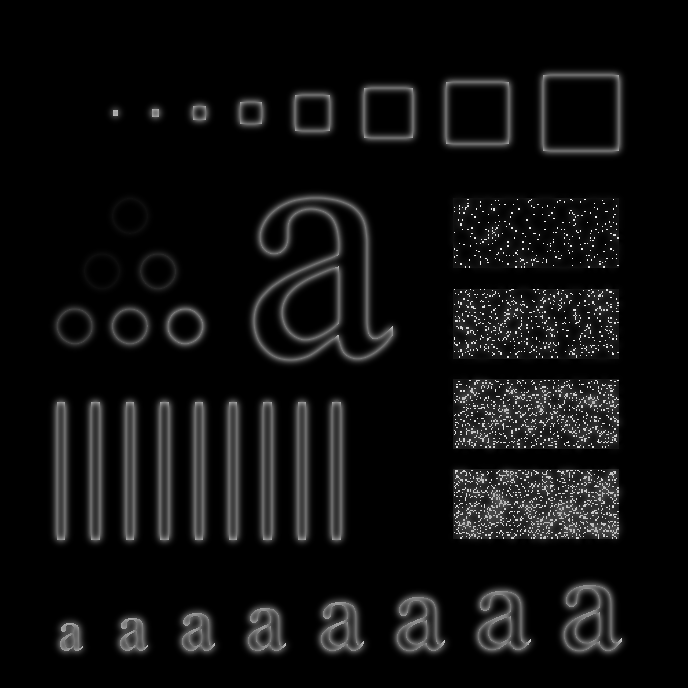
\includegraphics[width=\textwidth]{plots2/Q5_2_highpass_30.png}
         \caption{$\sigma=30$}
         \label{Q5_2_highpass_30}
     \end{subfigure}
     \hfill
     \begin{subfigure}[b]{.3\textwidth}
         \centering
         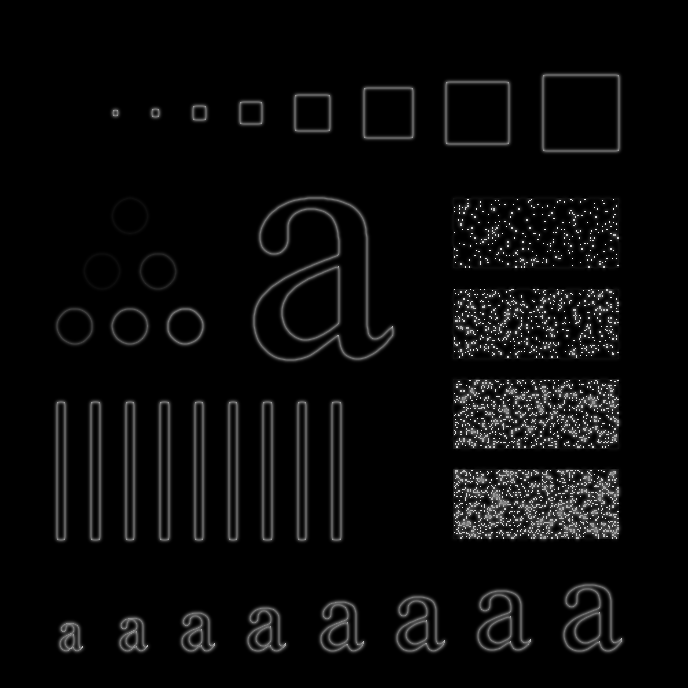
\includegraphics[width=\textwidth]{plots2/Q5_2_highpass_60.png}
         \caption{$\sigma=60$}
         \label{Q5_2_highpass_60}
     \end{subfigure}
     \hfill
     \begin{subfigure}[b]{.3\textwidth}
         \centering
         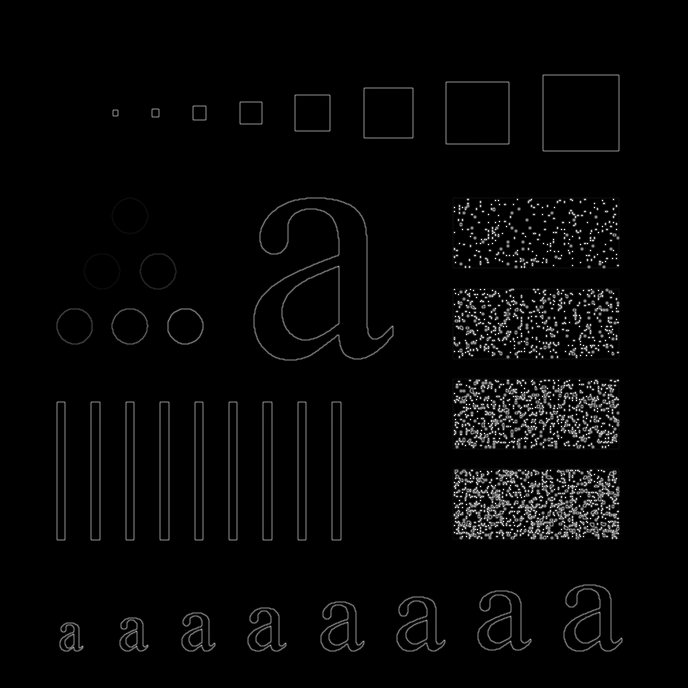
\includegraphics[width=\textwidth]{plots2/Q5_2_highpass_160.png}
         \caption{$\sigma=160$}
         \label{Q5_2_highpass_160}
     \end{subfigure}
     
    \caption{The Gaussian highpass filter and output images}
    \label{Gaussian highpass filter}
\end{figure}

With the increase of $\sigma$ more features in low frquency will be filtered, and finally only edge can be reserved.

\subsection*{Discussion} \

Interestingly, we found that while the addition of highpass filter and lowpass filter with same $\sigma$ produce an all-white image, the addition of the filtered image is equal to the original image. When $\sigma=1$, almost no feature remained after filtered by lowpass filter, which means no feature contained in the extreme low frquency, with more infromation in relatively high frquency remained, almost all the fertures remained, for highpass filter, only edge remained after most of the information in low frquency is removed. So we can draw a conclusion that, most of the information, except th edge, contained in low frquency domain.

We can also conclude the application of differnet kind of Gaussian filters. For Gaussian lowpass filter, with lower $\sigma$ we can remove the details in the image. For Gaussian highpass filter, with higher $\sigma$ we can remove most of the pixels except the edge.

\newpage
\section*{Task 3: Butterworth notch filters}

\begin{problem}
Implement the Butterworth notch filters to the input images Q5\_3.tif. Refer to slides 110 to 114 of Lecture 4.

\begin{figure}[H]
    \centering
    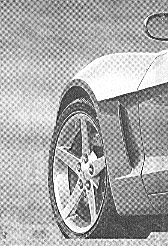
\includegraphics[width=0.3\linewidth]{plots/Q5_3.png}
    \caption{Q5\_3.tif}
    \label{Q5_3.tif}
\end{figure}

\end{problem}

\subsection*{Analysis} \
In this task, our goal is quite similar to that in Task 2, we want to reduce signal with speicfic frquency to , the Butterworth notch filters can be described as $$H(u,v)=\frac{1}{1+[D(u,v)/D_0]^{2n}}$$ as shown in Figure \ref{Butterworth.png} bigger n is, more signal in high frquency will be filtered, and compared with Gaussian filter, we found that with bigger n, wider range of signal in low frquency will be presevered.

Different from Gaussian filter, two papameter in butterworth filter can be adjusted, $\sigma$, the cutoff frquency and the $n$, the order, with bigger n, as shown in Figure \ref{Butterworth.png}, the information in high frquency domain will be absoultely filtered, with smaller n, some information in high frquency domain will be reserved and soem information in low frquency will be filtered.

\begin{figure}[H]
    \centering
    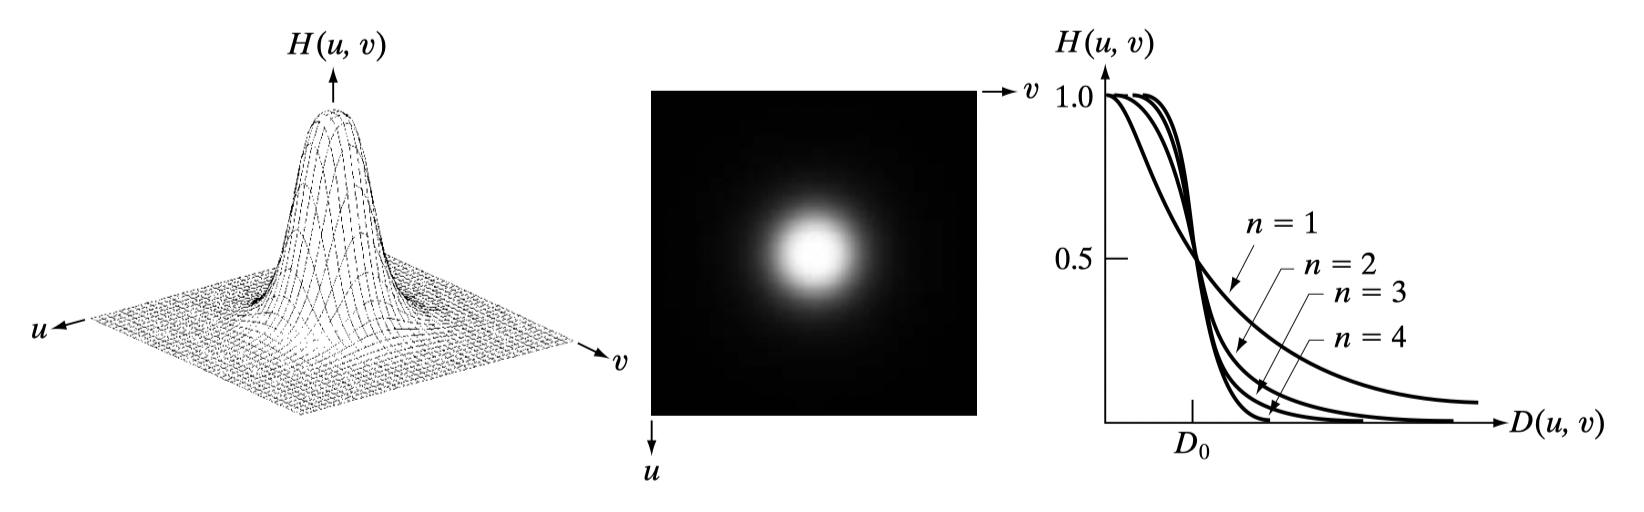
\includegraphics[width=0.8\linewidth]{chart/Butterworth.png}
    \caption{Butterworth lowpass filter}
    \label{Butterworth.png}
\end{figure}


For the given image we first apply the DFT to it, and we found that the noise is contained in 8 points, and our task is to remove them. We generate 8 Butterworth highpass filter, and add them together to obtain the filter shown in Fugure \ref{Butterworth filter}, then we apply it to the spectrum of the spectrum and get Figure \ref{Q5_3_spectrum_filtered_1_30}, then we will compare which parameters are better.

\begin{figure}[H]
    \centering
    \begin{subfigure}[b]{.3\textwidth}
         \centering
         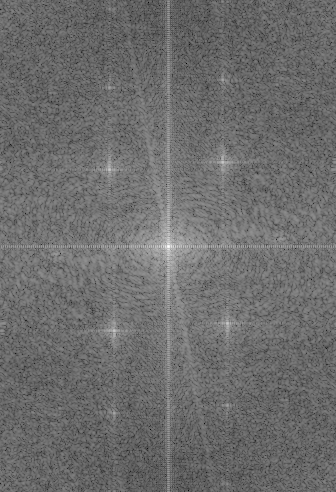
\includegraphics[width=\textwidth]{plots2/Q5_2_spectrum.png}
         \caption{Original image after DFT}
         \label{Q5_2_spectrum}
     \end{subfigure}
     \hfill
     \begin{subfigure}[b]{.3\textwidth}
         \centering
         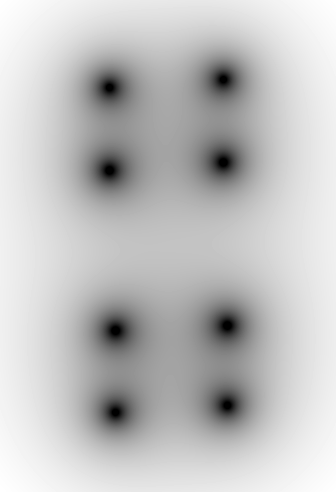
\includegraphics[width=\textwidth]{plots2/Q5_3_filter_1_30.png}
         \caption{Butterworth filter}
         \label{Q5_2_spectrum}
     \end{subfigure}
     \hfill
     \begin{subfigure}[b]{.3\textwidth}
         \centering
         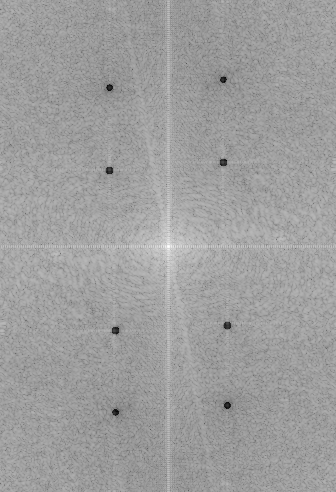
\includegraphics[width=\textwidth]{plots2/Q5_3_spectrum_filtered_1_30.png}
         \caption{Specturm after filtering}
         \label{Q5_3_spectrum_filtered_1_30}
     \end{subfigure}
    \caption{Butterworth filter}
    \label{Butterworth filter}
\end{figure}

\subsection*{Result} \

Here we apply Butterworth filter with differnet n and $\sigma$ to image.

\begin{figure}[H]
    \centering
        \begin{subfigure}[b]{.22\textwidth}
             \centering
             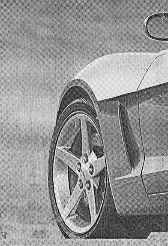
\includegraphics[width=\textwidth]{plots2/Q5_3_1_10.png}
             \caption{$n=1$, $\sigma=10$}
             \label{Q5_3_1_10}
         \end{subfigure}
         \hfill
         \begin{subfigure}[b]{.22\textwidth}
             \centering
             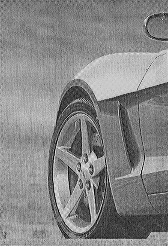
\includegraphics[width=\textwidth]{plots2/Q5_3_1_30.png}
             \caption{$n=1$, $\sigma=30$}
             \label{Q5_3_1_30}
         \end{subfigure}
         \hfill
         \begin{subfigure}[b]{.22\textwidth}
             \centering
             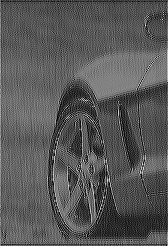
\includegraphics[width=\textwidth]{plots2/Q5_3_1_60.png}
             \caption{$n=1$, $\sigma=60$}
             \label{Q5_3_1_60.tif}
         \end{subfigure}
         \hfill
         \begin{subfigure}[b]{.22\textwidth}
             \centering
             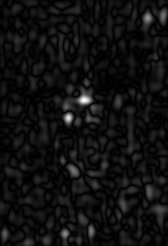
\includegraphics[width=\textwidth]{plots2/Q5_3_1_120.png}
             \caption{$n=1$, $\sigma=120$}
             \label{Q5_3_1_120.tif}
         \end{subfigure}
     \vfill
         \begin{subfigure}[b]{.22\textwidth}
             \centering
             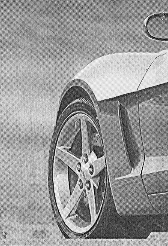
\includegraphics[width=\textwidth]{plots2/Q5_3_2_10.png}
             \caption{$n=2$, $\sigma=10$}
             \label{Q5_3_2_10}
         \end{subfigure}
         \hfill
         \begin{subfigure}[b]{.22\textwidth}
             \centering
             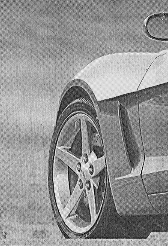
\includegraphics[width=\textwidth]{plots2/Q5_3_2_30.png}
             \caption{$n=2$, $\sigma=30$}
             \label{Q5_3_2_30}
         \end{subfigure}
         \hfill
         \begin{subfigure}[b]{.22\textwidth}
             \centering
             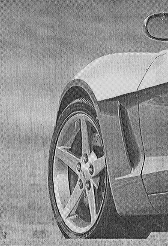
\includegraphics[width=\textwidth]{plots2/Q5_3_2_60.png}
             \caption{$n=1$, $\sigma=60$}
             \label{Q5_3_1_60}
         \end{subfigure}
         \hfill
         \begin{subfigure}[b]{.22\textwidth}
             \centering
             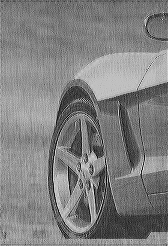
\includegraphics[width=\textwidth]{plots2/Q5_3_2_120.png}
             \caption{$n=2$, $\sigma=120$}
             \label{Q5_3_2_120}
         \end{subfigure}
     \vfill
         \begin{subfigure}[b]{.22\textwidth}
             \centering
             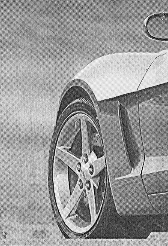
\includegraphics[width=\textwidth]{plots2/Q5_3_2_10.png}
             \caption{$n=3$, $\sigma=10$}
             \label{Q5_3_3_10}
         \end{subfigure}
         \hfill
         \begin{subfigure}[b]{.22\textwidth}
             \centering
             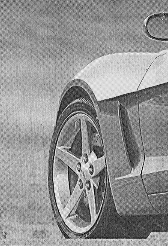
\includegraphics[width=\textwidth]{plots2/Q5_3_2_30.png}
             \caption{$n=3$, $\sigma=30$}
             \label{Q5_3_3_30}
         \end{subfigure}
         \hfill
         \begin{subfigure}[b]{.22\textwidth}
             \centering
             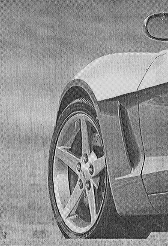
\includegraphics[width=\textwidth]{plots2/Q5_3_2_60.png}
             \caption{$n=3$, $\sigma=60$}
             \label{Q5_3_3_60.tif}
         \end{subfigure}
         \hfill
         \begin{subfigure}[b]{.22\textwidth}
             \centering
             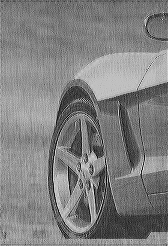
\includegraphics[width=\textwidth]{plots2/Q5_3_2_120.png}
             \caption{$n=3$, $\sigma=120$}
             \label{Q5_3_3_120.tif}
         \end{subfigure}
     \caption{Apply butterworth filter}
     \label{Butterworth filter}
\end{figure}

\subsection*{Discussion} \

We found that, with n = 1, we increase $\sigma$, when $\sigma=30$, most of the blemish disappeared, if we keep increase $\sigma$, the image begin to be damaged. For n = 2, blemish disappeared at $\sigma=60$, then image begin to be damaged, and for n=3, this number is bigger. We can find from Figure \ref{Butterworth filter} that with n=1 the buttereorth filter is similar to Gaussian filter, and for bigger n it is similar to ideal lowpass filter. So both increase n and $\sigma$ can let more signal in low frequency remain, and we also find that when most of the blemish is removed, smaller n can led to less damage to image.

So generally, if using butterworth filter to reduce the blemish in the figure, we can use small n so only a small area will be totally moved, and we need to use relative high $\sigma$ to make sure the blemish is removed.

\section*{Conclusion}

In this lab we applied sobel filter on both spatal and frequency domain, we use Gaussian and Butterworth lowpass and lowpass filter in frquency domain. 

Filtering in spatal domain focus on the relationship between pixels within a specific domain, and filtering in frquency domain focus on the speed pixels are chaning in all image and adjust the relationship. 

In my opinion, for remove unwanted signal from a image, we can use both spatal and frquency filtering, while filtering in frquency often have better performance, filtering in spatal domain require less computing, and for edge detection, I recommend to use spatal filter due to the error in digital calculating may cause bad disturb in the result.

\newpage
\section*{Source code}

\inputminted[linenos,breaklines, breakafter=d, bgcolor=bg]{python}{code/EE326_SUSTech.py}

\inputminted[linenos,breaklines, breakafter=d, bgcolor=bg]{python}{code/sobel_filter_11810818.py}

\inputminted[linenos,breaklines, breakafter=d, bgcolor=bg]{python}{code/gaussian_pass_11810818.py}

\inputminted[linenos,breaklines, breakafter=d, bgcolor=bg]{python}{code/butterworth_notch_filters_11810818.py}

\end{document}
